Para el escenario de funcionamiento off-grid necesitamos el coste del grupo
electrógeno, función de su potencia máxima activa.

Los datos de los modelos se han extraído de una página comercial
\footnote{\url{https://www.apmaquinaria.com/60-generadores-electricos-diesel}},
detallados en la tabla \ref{tab:generator_data}, cuya regresión lineal se
presenta en el gráfico \ref{fig:generator_regression}.

Usualmente se suele anunciar la potencia aparente de un generador diesel, pero
aquí estamos interesados en la potencia activa para nuestro balance de
potencias, así que hemos tomado un factor de potencia de 0.8, que por otra
parte es un valor dado frecuentemente cuando sí se publicita la potencia activa
del grupo.

\begin{table}[htbp]
	\centering
	\begin{tabular}{lrrr}
		\toprule
		Marca         & Modelo         & Potencia activa [kW] & Precio [\euro] \\
		\midrule
		ITC power     & DG10000SE-T    & 8                    & 2859           \\
		ITC power     & DG10000SE      & 8                    & 2690           \\
		Zipper        & ZI-STE6700DH   & 4                    & 945            \\
		ITC power     & 6100XE         & 5                    & 1070           \\
		ITC power     & DG6000LE       & 5                    & 1115           \\
		ITC power     & DG7800LE       & 6                    & 1215           \\
		Hyundai       & DHY6000LEK     & 5                    & 1400           \\
		ITC power     & DG6000SE       & 5                    & 1431           \\
		Hyundai       & DHY8500LEK     & 6                    & 1500           \\
		Kompak        & 8000LE-T       & 6                    & 1539           \\
		Black\&Decker & BXGND6300E     & 6                    & 1800           \\
		Kpc           & KDG12EA3       & 9                    & 3741           \\
		Kpc           & KDG12STA3      & 9                    & 5369           \\
		ITC power     & DG12000XSET    & 9                    & 5120           \\
		ITC power     & DG11KEm        & 10                   & 5250           \\
		Hyundai       & DHY12000XSE-T  & 9                    & 5400           \\
		ITC power     & DG22KE         & 16                   & 5580           \\
		Kpc           & KX16S          & 12                   & 7885           \\
		ITC power     & DG14KSE        & 10                   & 6369           \\
		Kompak        & KPCTW-11L      & 11                   & 6490           \\
		ITC power     & DG16KSE        & 12                   & 7050           \\
		Kpc           & KX20S3         & 14                   & 7900           \\
		Kompak        & KPCTW-11Li     & 11                   & 8000           \\
		Genergy       & GDS20T         & 16                   & 8177           \\
		Genergy       & GDS27M         & 21                   & 9874           \\
		Hyundai       & DHY22KSEm      & 22                   & 9995           \\
		Hyundai       & DHY45KSE       & 32                   & 12500          \\
		Genergy       & GDS70T         & 56                   & 13000          \\
		ITC power     & DG66KSE        & 48                   & 13669          \\
		ITC power     & DG110KSE       & 80                   & 16889          \\
		Kpc           & KX130S3        & 96                   & 17568          \\
		Genergy       & GDS200T        & 14                   & 25700          \\
		Ayerbe        & AY-1500-200 TX & 16                   & 35800          \\
		ITC power     & DG110KSE       & 80                   & 16900          \\
		Kpc           & KX130S3        & 10                   & 17500          \\
		Ayerbe        & 5419517        & 40                   & 17200          \\
		Kompak        & KPCTDW-110Li   & 88                   & 17700          \\
		Hyundai       & DHY110KSE      & 80                   & 19170          \\
		Hyundai       & DHY125KSE      & 90                   & 21900          \\
		\bottomrule
	\end{tabular}
	\caption{Modelos para grupos electrógenos.}
	\label{tab:generator_data}
\end{table}


\begin{figure}[h] \centering
	\centering
	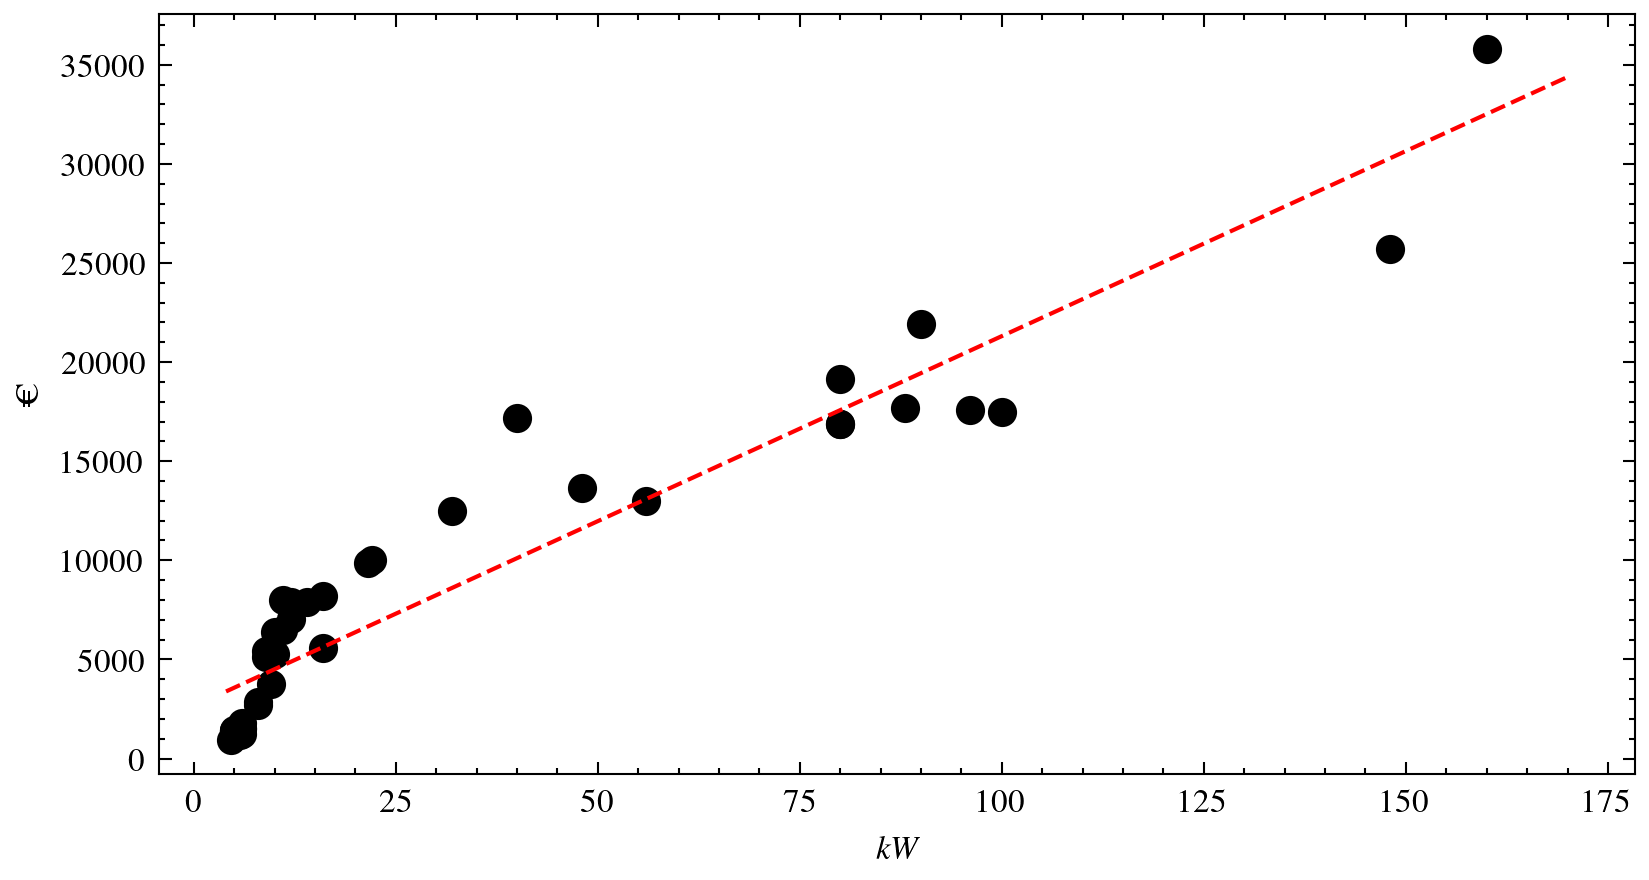
\includegraphics[width=1\textwidth]{./capitulos/adquisicion_de_datos/images/generator_regression.png}
	\caption{Ajuste lineal de precios para generador diesel.}
	\label{fig:generator_regression}
\end{figure}


\begin{equation}
	\text{coste\_generador} \left[\frac{\text{\euro}}{kW}\right] = 2637.29 + 186.73 \cdot P_{red_{max}}
\end{equation}

donde $P_{red_{max}}$ es la potencia máxima del grupo electrógeno, pero lo
hemos indicado como potencia máxima de red, porque en el estudio de sistema
off-grid, consideramos que el generador diesel sustituye a la red.
